\documentclass[en]{../../../../../../eplexam}

\usepackage{../../../../../../eplunits}

\hypertitle{Radiation and communication systems}{7}{ELEC}{2795}{2019}{Janvier}{All}
{Alice Borbath \and Olivier Leblanc \and Maxime Wattiaux}
{Cristophe Craeye, Danielle Janvier, Jérome Louveaux, Claude Oestges and Luc Vandendorpe}

\section{(4,5 points)}

Frequency: $f=\SI{75}{GHz}$.

\begin{figure}[ht!]
    \centering
    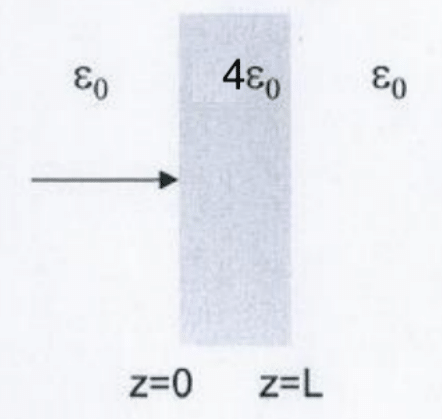
\includegraphics[scale=0.4]{Q1.png}
\end{figure}

\begin{enumerate}
    \item (1 point) Calculate the reflection coefficient at $z=0$.
    \item (1 point) Calculate the smallest value of $L$ such that there is total transmission at $z=0$ (in mm).
    \item (2,5 points) Assume that the frequency is not exactly at \SI{75}{GHz}, calculate the percentage of reflected power.
    Consider the frequency equal to $f=f_0(1+\delta)$ and develop to the first order of $\delta$.
    
    Hint: use $\sin(\pi+\epsilon)=-\sin(\epsilon)\approx-\epsilon$ and $\cos(\pi+\epsilon) \approx -1$.
\end{enumerate}

\nosolution

\section{(4,5 points)}

A wireless horizontal link is established over 100 meter distance at \SI{2.4}{GHz}. In first instance, we will assume that the antennas are placed high enough to be able to omit the effect of interaction with the ground. On the transmit side, the antenna is actually made of an array of two parallel half-wave dipoles, oriented perpendicularly to the ground and space by half a wavelength. The power fed to the pair of antennas is assumed to be split equally between the antennas, and matching at the common feeding part is supposed perfect. On the receiving side, an antenna with circular polarization, with 10dB gain is used. The antenna is correctly pointed and its pattern falls of by 3 dB at an angle close to 25 degrees from boresight. That antenna is badly matched: it has an impedance of $100-20j$ $\Omega$, while the receiver has \SI{50}{\Omega} input impedance. Its noise figure is also relatively bad, corresponding to 4 dB. The transmitted array is not well pointed towards the receiving antenna, because of non-equal phases in the two excitations, such that the pattern is actually pointing 20 degrees away from the line of sight. The noise contributed by the environment will be calculated assuming a \SI{290}{K} temperature in all directions and the occupied bandwidth is \SI{20}{MHz}.

\begin{figure}[ht!]
    \centering
    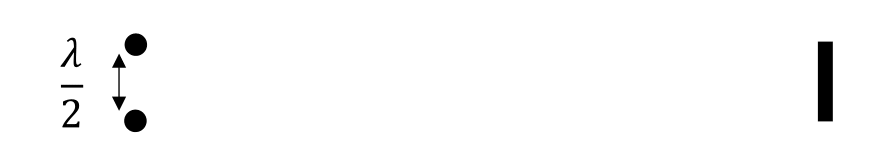
\includegraphics[scale=0.5]{Q2.png}
\end{figure}

\begin{enumerate}
    \item (4 points) Considering \SI{1}{mV} for the transmitting power, what is the SNR (in dB) observed at the receiver?
    \item (0,5 points) Please try to provide a rough estimate for an upper bound (in dB) of the (significant) effect of reflection on the ground, considering that the heights of the antennas above the ground are 20 meter.
\end{enumerate}

\nosolution

\section{(4,5 points)}

Wireless transmission QPSK between 1 TX and 2 RX. The signal at antenna $i$ (1 or 2) is 
\[                                                                                    
    y_i(t)=h_i\sum_{n=0}^{N-1} I_nu(t-nT)+w_i(t)
\]
where 
\begin{itemize}
    \item $h_i$ is the fading coefficient between Rx and Tx;
    \item $I_n$ is the complex symbol sent at instant $nT$;
    \item $u(t)$ is the transmit filter;
    \item $w_i(t)$ is the complex envelope of the AWGN corrupting the signal, with bandpass power spectral density $\frac{N_i}{2}$. The noise between different Rx is uncorrelated.
\end{itemize}
We consider the detection operation to be performed by containing the two signals $y_1(t)$ and $y_2(t)$ to recover the transmitted data. We first apply a matched filter operation on signals $y_i(t)$ with a filter having impulse response $u^*(-t)$, and we sample the output at positions $mT$. This produces samples $y'_i[m]=h_iI_m\epsilon_u+w'_i[m]$ where $\epsilon_u$ is the energy contained in $u(t)$.
\begin{enumerate}
    \item Assuming first that $\frac{N_i}{2}=\frac{N_0}{2}$ for all $i$, (3 points)
    \begin{itemize}
        \item What is the decision rule corresponding to the ML estimate of $I_m$ based on both $y'_1[m]$ and $y'_2[m]$? Remark: don't forget $I_m$ is complex. Hint: find the ML estimate for the real part and the imaginary part.
        \item What can you say about the SNR of the decision variables? Comment please.
    \end{itemize}
    \item Let us consider that all $N_i$ can be different (1,5 points),
    \begin{itemize}
        \item Calculate again the ML decision rule for the data. 
        
        Hint: multiply each $y'[m]$ by a well-chosen term in order to obtain noise terms with equal variance.
        \item What can you say about the SNR of the decision variables compared to the SNR associated with each receive antenna? Comment please. What happens when for instance $N_1$ is much larger than $N_2$.
    \end{itemize}
\end{enumerate}

\nosolution

\section{(4,5 points)}

\begin{enumerate}
 \item 
If we consider a Ricean fading channel described
\begin{itemize}
    \item by a dominant multipath with a specific angle-of-arrival
    \item by a Rayleigh made of a large number of multipath arriving at the mobile terminal in the horizontal plane from all directions in azimuth.
\end{itemize}
In that case, the Doppler spectrum is given by:
\begin{enumerate}
    \item the so-called Jakes spectrum defined by 
    \[
     (v) = \left\{ \begin{array}{ccc}
                  \frac{3}{2 \pi v_m \sqrt{1 - \frac{v^2}{v_m^2}}} & \textrm{for} &  |v| < v_m \\
                  0 & \textrm{for} & |v| \ge v_m
                  \end{array} \right.
    \]
    where $v_m$ is the maximum Doppler shift.
    \item a weighted combination of the Jakes spectrum and a delta function at the origin
    \item a weighted combination of the Jakes spectrum and a delta function centered at an adequate Doppler frequency
    \item a weighted combination of the so-called Jakes spectrum and a flat spectrum
\end{enumerate}

\item
In an hexadecimal cellular network characterized by a path-loss exponent equal to 3, a signal to interference ratio of 10 dB is targeted. The frequency reuse pattern must be based on at least 
    \begin{enumerate}
        \item 4 Cells
        \item 7 Cells
        \item 11 Cells
        \item 19 Cells
    \end{enumerate}

\item A cellular system operates in a Rayleigh fading channel such that the symbol period is smaller than the channel delay-spread. This implies that:
    \begin{enumerate}
        \item the channel creates inter-symbol interferences
        \item the channel transfer function is flat over the system bandwidth
        \item the coherence time of the channel cannot be defined
        \item the channel transfer function is real-valued
    \end{enumerate}

\item
Waveguiding propagation mechanisms (in corridors or street canyons) mostly cause
    \begin{enumerate}
        \item a large shadowing
        \item frequency selectivity
        \item a reduced Doppler frequency
        \item a path-loss exponent equal to 4
        \item a path-loss exponent lower than 2
    \end{enumerate}
    
\item
Suppose an electromagnetic wave coming from a transmitter with a circular polarization is propagating in a long street with high buildings. What is the best denomination for the polarization of the reflected wave? 

\begin{enumerate}
    \item circular
    \item elliptical
    \item horizontal linear
    \item vertical linear
    \item oriented linear 
\end{enumerate}

\item
In order to have the best VDSL system (best transmission), what can we say about cables? They must be:
    \begin{enumerate}
        \item no cables (wireless communication)
        \item shorter and thinner
        \item shorter and thicker
        \item longer and thinner
        \item longer and thicker
    \end{enumerate}
    
\item
What is the main advantage of OFDM that we can't find in DMT modulation?
    \begin{enumerate}
        \item Adapting the constellation size of each tone to SNR
        \item Permet d'implémenter facilement FDD
        \item Taking benefit from frequency diversity
        \item \dots
        \item \dots
    \end{enumerate}
    
\item
What is the main purpose of twisted-pair wires?
\begin{enumerate}
    \item Reduce interferences for the differential mode
    \item Reduce interferences for the common mode
    \item Reduce the attenuation of the signal along its path
    \item Insert the wire more easily in the \dots
    \item Help for vectoring
\end{enumerate}

\item
Radio frequency interference (RFI):
\begin{enumerate}
    \item Signal with high power that affects all xDSL systems
    \item Signal with high power that \dots
    \item Signal with low power \dots
    \item Signal with low power \dots
    \item Signal with low power \dots
\end{enumerate}

\end{enumerate}

\nosolution

\end{document}
